\section{Pipeline characteristics}
\subsection*{Number of stages}
\hspace{\parindent}The Cortex-A72 processor has a variable-length pipeline, the minimum length of which is 15 stages. This is a result of the different functional units included in the CPU, and so the maximum pipeline length can vary in other ARMv8-based processors. \cite{pipeline} The A72's pipeline is, for the most part, the same as that of its predecessor, the Cortex-A57.
\subsection*{Names}
\hspace{\parindent}To simplify the the pipeline model, its stages can be divided into 5 groups and named according to the functional units that perform them: \cite{pipeline}
\begin{itemize}
	\item \textbf{Fetch}, during cycles 1-5.
	\item \textbf{Decode}, during cycles 6-12.
	\item \textbf{Issue}, in cycle 13.
	\item \textbf{Execute}, during the following cycles, depending on the required execution units; integer and branch operations take the shortest, at only one cycle.\footnote{This stage is the only significant difference between the Cortex-A72's pipeline and the A57's, whose functional units exhibit deeper pipelines.}
	\item \textbf{Retire}, or commit, in the last cycle.
\end{itemize}
\hspace{\parindent}
\begin{figure}[H]
	\begin{center}
		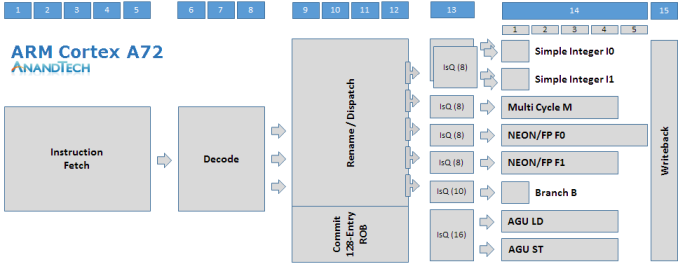
\includegraphics[width=0.7\linewidth]{imgs/a72pipeline.png}
		\caption{The structure of a Cortex-A72 processor core}
	\end{center}
\end{figure}
\pagebreak{}
\section{Steps of instruction execution}
\subsection*{Fetch}
\hspace{\parindent}Instruction execution begins as up to three instructions are fetched from the L1 instruction cache. For branch instructions, prediction also takes place during this stage, making use of the BTB and static predictor this architecture provides.
\subsection*{Decode}
\hspace{\parindent}In this next stage, the previous instructions are decoded into micro-operations to be fed into the execution units, register renaming is performed, removing any potential WAW or WAR hazards, and up to five of the decoded micro-ops are dispatched to the issue queues; this stage could therefore be interpreted as three separate ones (decode, rename and dispatch), with the first taking four cycles, and the latter two taking two cycles each.\par
Performing register renaming is key in order to facilitate out-of-order execution in the following stages. It should also be noted that, prior to the renaming, the instructions operate on a virtual register pool, which helps to prevent the number of registers specified at the architectural level from becoming a bottleneck. \cite{renaming}
\subsection*{Issue}
\hspace{\parindent}Once they have entered the issue queue, the micro-operations are scheduled onto their respective execution units, up to eight at a time, corresponding to the eight execution units of this processor. From this point on, instruction execution is performed out-of-order.
\subsection*{Execute}
\hspace{\parindent}This stage is different for each instruction, due to the different execution units that perform this step. Here it is worth noting that some of the more common operations (basic integer operations, vector operations, and load/stores, in this case) have two available execution units, in order to avoid structural hazards.
\subsection*{Retire}
\hspace{\parindent}Finally, once all the micro-ops of a given instruction have finished executing, its result is written to a 128-entry re-order buffer, and then sent back to the dispatch unit to update the register files and commit the instructions in order.
\pagebreak{}
\section{Performance studies}
\hspace{\parindent}The main contributors to the increased performance of the Cortex-A72 compared to the previous A57, from an architectural standpoint, are the new branch predictor, the increased decode/dispatch operation bandwidth, and modified execution units. \par
These changes contribute to more efficient use of the predictor units, as well as up to 20\% more accurate predictions, a more continuous influx of micro-operations to the execution units, lower latencies for floating-point and SIMD operations, and up to 30\% faster fetching of data from cache thanks to the combined L1/L2 prefetcher, among other improvements which could be seen in figures \ref{cortexA72performance}, \ref{cortexA72power}, and \ref{cortexA72usable} earlier. \cite{androidauthority} \par
The performance of the Cortex-A72 can be studied further using a Raspberry Pi 4, as its system on chip, the Broadcom BCM2711, implements it as its only CPU. This makes it easier to isolate the results compared to other SoCs which include a second, less powerful CPU, following ARM's big.LITTLE design, often used in smartphones for the increased power efficiency that it can provide in that use case. Taking this into account, here are some benchmark results for the aforementioned system:
\subsection*{Linpack}
\hspace{\parindent}A classic benchmark program for testing floating point performance, the results in figure \ref{linpack} of the Linpack benchmark show the increase in performance, of nearly four times the amount of instructions per second, of the A72 compared to the Cortex-A53, used in the Raspberry Pi 3, despite only running 100 MHz faster: \cite{linpack}
\begin{figure}[H]
	\begin{center}
		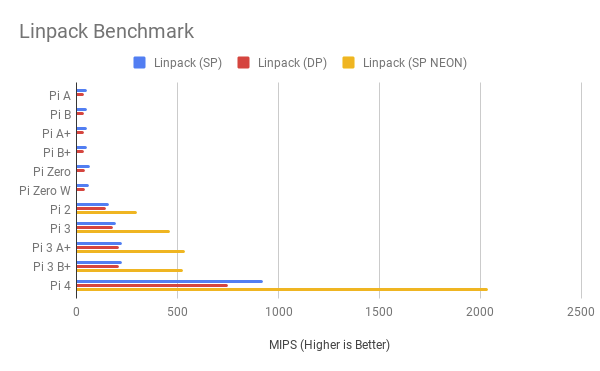
\includegraphics[width=0.7\linewidth]{imgs/linpack.png}
		\caption{Linpack benchmark results for different models of Raspberry Pi}
		\label{linpack}
	\end{center}
\end{figure}
The previous figure also shows the progression in performance from the ARMv6-based ARM11 CPU of the first Raspberry Pi, through the ARMv7-based Cortex-A7 of the Pi 2.
\subsection*{SysBench}
\hspace{\parindent}This benchmark software is based around multi-threaded prime number computation. In this case, as shown in figure \ref{sysbench}, the A72 is faster than the A53 of the Raspberry Pi 3, but the margin is not as large as with Linpack, this time showing a performance improvement of about 36\% when testing for prime numbers below 20000: \cite{sysbench}
\begin{figure}[H]
	\begin{center}
		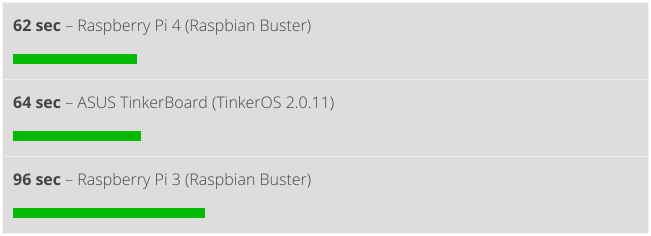
\includegraphics[width=0.7\linewidth]{imgs/sysbench.png}
		\caption{Sysbench results for the Pi 4, Pi 3 and ASUS TinkerBoard}
		\label{sysbench}
	\end{center}
\end{figure}
The ASUS TinkerBoard also shown in the graph, for reference, uses the ARMv7-based Cortex-A17 processor included in the Rockchip RK3288 SoC, running at 1.8 GHz, 400 MHz faster than the Pi 4's A72. The A17 was the last ARM-designed CPU using the ARMv7 architecture, and as seen here, can be superseded at lower clock speeds by the newer processors.